Shortbus ist ein Programm (Desktopanwendung) welches in der seriellen- aber auch Netzwerkkommunikation zum Einsatz kommt. 

Es handelt sich bei Shortbus um ein Modbus RTU und Modbus TCP/IP Scanner.
Dabei ist die Hauptaufgabe bei der seriellen Kommunikation das Auslesen und Einschreiben von Werten in das Modbus Register welcher einer Client/Server Architektur folgt.


Das Programm unterstützt neben dem Auslesen und Einschreiben von Werten in Modbus Register auch das  automatische Einschreiben in ein Modbus Register (Zweck: automatische Testung einer Client/Server Verbindung)

Shortbus unterstützt noch andere Funktionen (Netzwerkfunktionen), doch diese sind in der seriellen Kommunikation nicht relevant. 
\cite[vgl.][]{software.informer:2024}

\subsection{Shortbus allgemeiner Teil}
Shortbus lässt sich in 2 große Bereiche gliedern. siehe Abb.~\ref{fig:Shortbusfenster}. 

Im oberen Teil von Shortbus erfolgen die gesamten Eingaben was das System (Client/Server) angeht:
\begin{itemize}
	\item Connection: Das ist die Art wie man sich mit dem System verbinden möchte. Man unterscheidet hierbei meist zwischen TCP (Transmission Control Protocol) oder COM (Schnittstelle am Laptop meist COM7)
	
	\item Node Adresse: Ist die Adresse, welche vom Bauteil verwendet wird. Jedes Bauteil (\zB QBM oder EBM-Papst) hat eine eigene Node Adresse.
	
	\item Starting Address: Diese bestimmt das erste Register was Ausgelesen werden soll. Die Register und deren Adressen können wie folgt angegeben werden:
		\begin{itemize}
			\item ob das Register bei null anfängt (0-Based) oder nicht
			\item wie das Register angegeben ist Hexadezimal (Hex) angegeben wird oder nicht
		\end{itemize}
	\item Length To Read: Gibt an wie viele Register ausgelesen werden. 
	\item Read Function: Hier wird die Registerart angegeben.
\end{itemize}

Im unteren Teil erfolgt die Ausgabe der einzelnen Modbus Register. Abb.~\ref{fig:Shortbusfenster}. 

\begin{figure}[H]
	\centering
	\includegraphics[width=1\linewidth]{Bilder/shortbus_fenster}
	\caption{Shortbus Desktopanwendung} 
	\label{fig:Shortbusfenster}
\end{figure}
  

\subsection{Shortbus Anwendung (Registerauslesung in der Entwicklungs- \ac{rltanlage})}

In der Entwicklungs- \ac{rltanlage} wird die Schnittstelle COM7 (USB-Port des Laptops) verwendet um eine Kommunikation (Connection) mit dem Modbus aufzubauen. Dabei wird der Modbus per Kabel  Abb.~\ref{fig:modbus_usbkabel} erweitert und mit dem Laptop und dessen USB-Schnittstelle verbunden.

\begin{figure}[H]
	\centering
	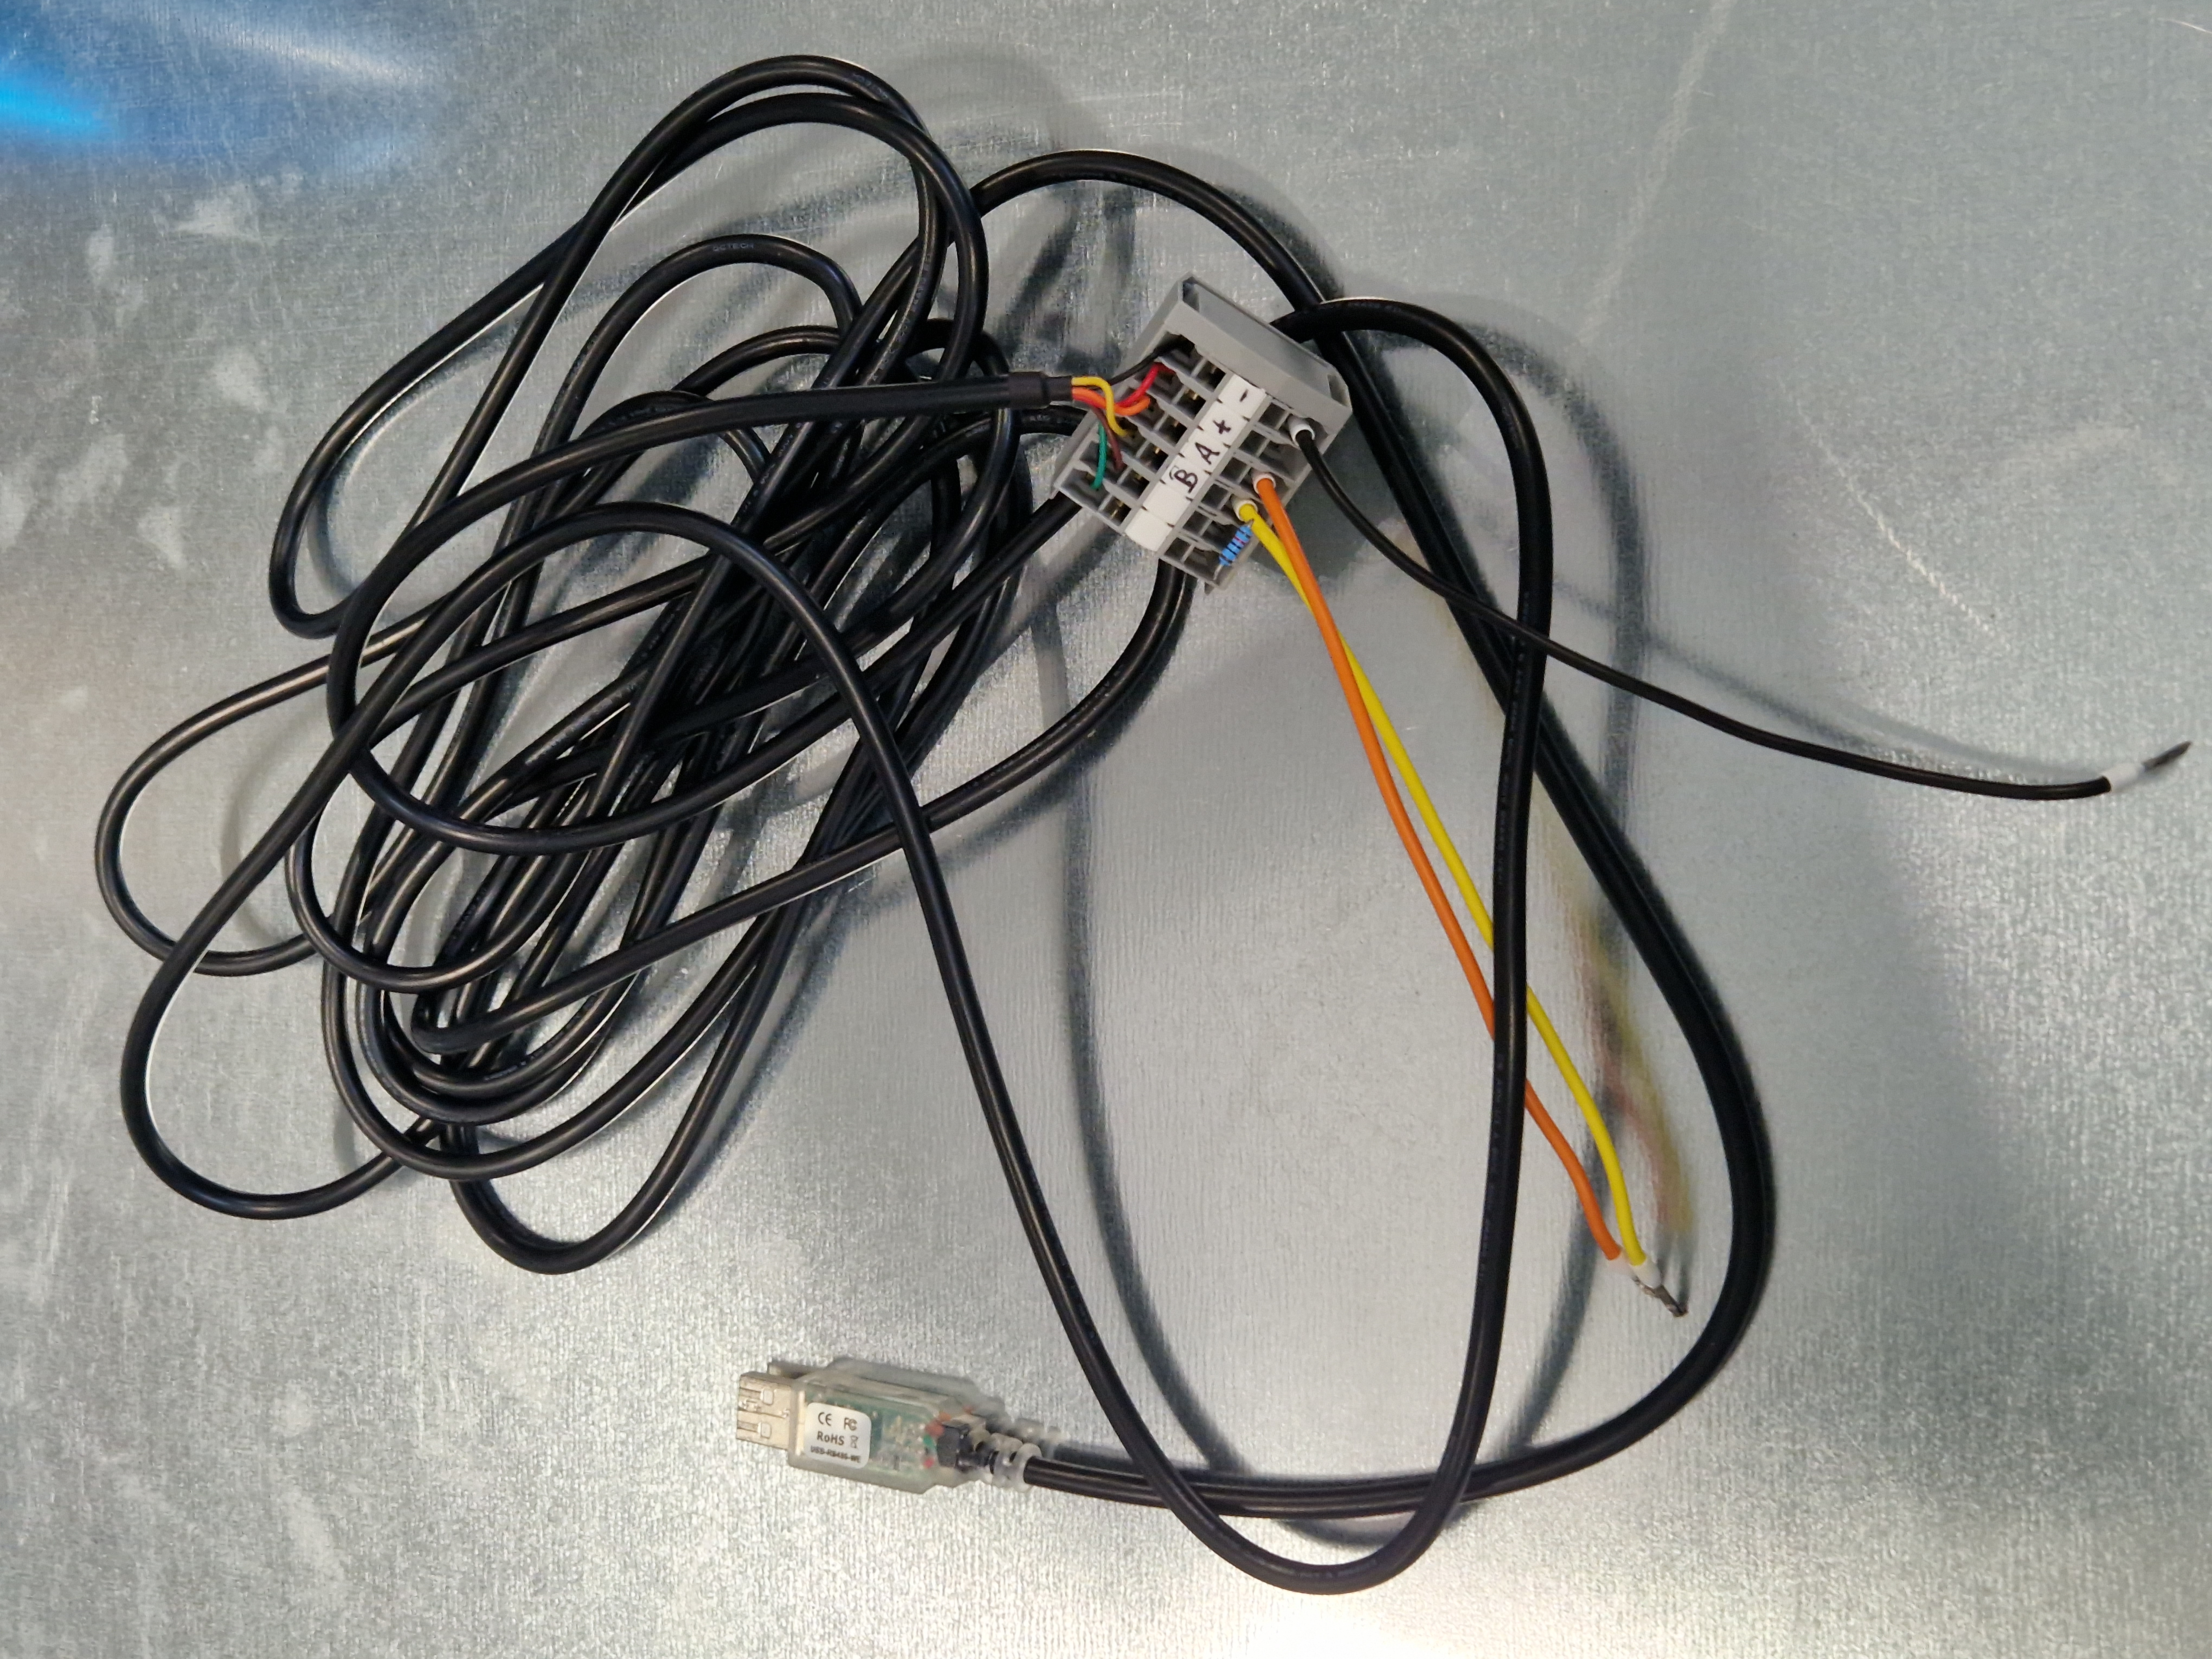
\includegraphics[width=0.5\linewidth]{Bilder/modbus_usbkabel}
	\caption{Modbus USB-Kabel} 
	\label{fig:modbus_usbkabel}
\end{figure}

 Danach werden die Einzelnen Komponenten der seriellen Kommunikation angegeben:
\begin{itemize}
	\item Baudrate (9600)
	\item Parity (Even)
	\item Stop Bits (1)
	\item Node Adresse (2)
	\item Starting Address 1 (Register fängt bei eins an und ist in nicht in Hexadezimal angegeben)
	\item Length To Read (Die ersten 85 Werte sollen ausgegeben werden)
	\item Read Funktion (FC 3 - Holding Register)
\end{itemize}

Beschreibung der Werte und Funktion von: Baudrate, Parity, Stop Bits, Read Funktion siehe \ref{modbus_funktionsweise}.



Abb.~\ref{fig:Shortbusausgabe}. 

\begin{figure}[H]
	\centering
	\includegraphics[width=1\linewidth]{Bilder/shortbus_ausgabe}
	\caption{Shortbus in Entwicklungsphase} 
	\label{fig:Shortbusausgabe}
\end{figure}


\subsection{VOR ABGABE LÖSCHEN}
%Umsetzung von Shortbus
%allgemein was kann das programm:

%wie lese ich daten aus
%das tdot / entwicklungsgerät 